\documentclass[11pt, letterpaper]{article} % Copyright (c) 2020 Brian Schubert


\def\LABnumber{5}
\def\LABtitle{Introduction to Quartus}
\def\LABdatedue{August 12th, 2020}
\def\LABdatesubmitted{August 12th, 2020}
\def\LABabstract{\small This lab served as an introduction to designing combinational logic circuits. Intel's Quartus Prime programmable logic design software was used to develop half-adder, full-adder, and 8-bit adder circuits. These circuits were tested both by mapping them onto the DE1-SoC board's FPGA, and by using the simulation tools provided by Quartus.}

% ECEE 2160 Lab Report Header
%
% Copyright (c) 2020 Brian Schubert
% 
% This header file was created to format lab reports in my
% Embedded Design course taken Northeastern University during
% the Summer 2 2020 semester.
%

% Many packages are retained from previous lab report headers
% for future convenience. 
\usepackage{amsmath,amsfonts,amssymb,amsthm}
\usepackage[english]{babel}
\usepackage{caption}
\usepackage[makeroom]{cancel}
\usepackage[dvipsnames,table]{xcolor}
\usepackage[inline]{enumitem}
\usepackage{esint}
\usepackage{fancyhdr}
\usepackage{geometry}
\usepackage{graphicx}
\usepackage{hyperref}
\usepackage[utf8]{inputenc}
\usepackage{listings} % For code listings
% Replace times with this package to typeset math in times aswell
% Note: no bold typeface exists for the times font, so \boldsymbol
% does not work when using a times font in math mode.
%\usepackage{mathptmx}
\usepackage{mathtools}
\usepackage{multicol}
\usepackage{multirow}
\usepackage{pgfplots}
\usepackage{placeins} % For FloatBarrier
\usepackage{siunitx}
\usepackage{subcaption}
\usepackage{tikz}
\usepackage[american]{circuitikz}
\usepackage{todonotes}
\usepackage{times} % For times font
\usepackage[explicit]{titlesec}

% Use deja-vu sans mono for monospaced typeface
% Must be after times font package.
\usepackage[scaled=0.9]{DejaVuSansMono}

\geometry{left=1in,right=1in,top=1in,bottom=1in}

% File prefixes to use when searching for graphics.
\graphicspath{ {../images/} {./images/} }

% Color all used links blue.
\hypersetup{
    colorlinks=true,
    linkcolor=MidnightBlue,   
    citecolor=MidnightBlue,   
    urlcolor=MidnightBlue,
}

\urlstyle{same} % Print URLs using the surroudning font instead of forcing monospace

% Add headings from lab report template
\pagestyle{fancy}
\lhead{\LABauthor\\\LABcourse}
\rhead{\LABcoursetitle\\Lab Assignment \LABnumber}

% Macro to generate the an IPL template style title page
\newcommand{\makelabtitle}{
\begin{titlepage}
    \begin{center}
    \renewcommand{\baselinestretch}{1.2}
    
    % See https://tex.stackexchange.com/questions/252040/unwanted-border-around-the-image
    % for details on how to fix border due transparent cropped region in png.
    
\includegraphics[width=0.7\textwidth]{northeastern-header-cropped}\par
    
    \vspace{0.6in}

    {
        \renewcommand{\baselinestretch}{1.2}
        \Large
        \LABcourse\par
        \LABcoursetitle\par
        \LABsemester\par
    }

    \vspace{0.3in}

    {\LARGE\bfseries
       \LABreportheading{} \LABnumber\par
        \ifx \LABtitle \undefined
        \else
            \LABtitle\par
        \fi
    }
    
    \vspace{0.3in}
    
    {
        \Large
        \LABauthor\par
        \ifx \LABauthoremail \undefined
        \else
            \large \texttt{\LABauthoremail}\par
        \fi
    }

    \vspace{0.4in}
    
    {
        \large
        \setlength{\tabcolsep}{4pt}
        \begin{tabular}{>{\bfseries}rl}
            Instructor:     & \LABinstructor\\
            Due Date: 	    & \LABdatedue\\
            Submitted:      & \LABdatesubmitted\\
        \end{tabular}
        
    }

    \end{center}
    \ifx \LABabstract \undefined
    \else
        \vfill\null
        \begin{abstract}
            \LABabstract
        \end{abstract}
    \fi
\end{titlepage}
}

% Common defaults for lab report title page
\def\LABcourse{ECEE 2160}
\def\LABcoursetitle{Embedded Design: Enabling Robotics}
\def\LABsemester{Summer 2 2020}
\def\LABauthor{Brian Schubert}
\def\LABauthoremail{schubert.b@northeastern.edu}
\def\LABinstructor{Syed Shazli}
\def\LABreportheading{Report for Lab Assignment}


% Notation Definitions
\newcommand{\dd}[1]{\mathrm{d}#1}
\newcommand{\diffop}[2][]{\frac{\dd#1}{\dd #2}}
\newcommand{\pdiffop}[2][]{\frac{\partial #1}{\partial #2}}
\newcommand{\bvec}[1]{{\vec{\boldsymbol{#1}}}}
\newcommand{\relerr}[1]{\frac{\delta #1}{#1}}
\newcommand{\unitvec}[1]{\hat{\boldsymbol{#1}}}

\sisetup{inter-unit-product =\cdot}
\sisetup{per-mode = symbol}
\sisetup{separate-uncertainty = true}
\sisetup{multi-part-units=single}
\DeclareSIUnit{\radian}{rad}
\DeclareSIUnit{\degreeFahrenheit}{{}^\circ F}

% Use computer modern roman fontface for emf symbol.
% https://tex.stackexchange.com/questions/67881/resetting-mathcal-font-to-default
\DeclareMathAlphabet{\defaultmathcal}{OMS}{cmsy}{m}{n}
\newcommand{\emf}{\defaultmathcal{E}}



% Print table and figure labels in bold font
\captionsetup[table]{labelfont=bf}
\captionsetup[figure]{labelfont=bf}

%\captionsetup[lstlisting]{ format=listing, labelfont=white, textfont=white, singlelinecheck=false, margin=0pt, font={bf,footnotesize} }
\captionsetup[lstlisting]{labelfont=bf}

% Make table columns slighly wider by default
\setlength{\tabcolsep}{8pt}

% Custom code color scheme
\definecolor{codekeyword}{RGB}{3,0,130}
\definecolor{codeidentifier}{RGB}{20, 20, 80}
\definecolor{codestring}{RGB}{72, 140, 2}
\definecolor{codecomment}{rgb}{0.3,0.3,0.3}
\definecolor{codedirective}{RGB}{160, 130, 60}


% Custom listings styling
\lstdefinestyle{labreportstyle}{
    % Syntax highlighting
    basicstyle=\ttfamily\footnotesize,
    backgroundcolor=\color{gray!5},
    commentstyle=\itshape\color{codecomment},
    keywordstyle=\bfseries\color{codekeyword},
    stringstyle=\bfseries\color{codestring},
    identifierstyle=\color{codeidentifier},
    % Tab width and display
    tabsize=4,
    showtabs=true,
    % Don't show spaces in strings
    showspaces=false,
    showstringspaces=false,
    % Show line numbers
    numbers=left,
    numberstyle=\scriptsize\sffamily\color{gray},
    % Allow listing to break long lines
    breaklines=true,
    breakatwhitespace=true,
    % Frame settings
    frame=lines,
%    frame=bottomline,
    % Misc
    captionpos=t,
    keepspaces=true,
    xleftmargin=2mm,
    framexleftmargin=2mm,
}

% C++ specific styling
\lstdefinestyle{labreportstyle-C++}{
    language=C++,	% Not sure if redundant now, but was required at one point
    style=labreportstyle,
    directivestyle={\color{codedirective}},
    morekeywords={constexpr,nullptr,noexcept,static\_assert,alignof}
%    frame=bottomline,
}

% shell specific styling
\lstdefinestyle{labreportstyle-sh}{
    language=sh,
    style=labreportstyle,
    numbers=none,
    identifierstyle=\color{black},
    emph={\$},
    emphstyle=\bfseries\color{codekeyword},
}

% Conveience macro to load code file listings.
%
% Note that the style is automatically selected based on the language paramater.
\newcommand{\includecode}[2][C++]{%
    \lstinputlisting[caption={\texttt{#2}}, label={lst:#2}, language=#1, style=labreportstyle-#1]{#2}
}


\usepackage{floatpag} % for thisfloatpagestyle
\usepackage{pdflscape}

\begin{document}
\makelabtitle

\section*{Introduction}

This lab was an introduction to using Quartus to design combinational logic circuits. Half-adder and full-adder circuits were designed using the Quartus block diagram editor. These circuits were then mapped onto the DE1-SoC board's FPGA, and their behavior was verified by interacting with the board's I/O devices. The full-adder circuit was then used to develop an 8-bit adder circuit, which was tested using Quartus' circuit simulation tools. 

\section*{Lab Discussion}

\subsection*{Materials}

The following materials were used to complete this lab.
\begin{enumerate}
    \item Host computer (Linux Mint 19.3, x86\_64)
    \item DE1-SoC board (de1soclinux, armv7l)
\end{enumerate}
\subsection*{Software}
Intel's Quartus Prime Lite Edition (version 20.1) was installed on the host machine.

\subsection*{Prelab Assignment}

The prelab assignment consisted of preparing truth tables and circuit diagrams for the half- and full-adder circuits.

\begin{table}[h]\centering
    \caption{Prelab Truth Tables.}
    \def\arraystretch{1.2}
    \begin{subtable}[t]{0.48\linewidth}\centering
        \caption{Half-Adder}
        \begin{tabular}{|cc|cc|}
            \hline
            \multicolumn{2}{|m{1.5cm}|}{\bfseries\centering Inputs} & 
            \multicolumn{2}{m{1.5cm}|}{\bfseries\centering Outputs}\\
            $\boldsymbol{A}$ & $\boldsymbol{B}$ & $\boldsymbol{C}$ & $\boldsymbol{S}$\\
            \hline
            0 & 0 & 0 & 0\\
            0 & 1 & 0 & 1\\
            1 & 0 & 0 & 1\\
            1 & 1 & 1 & 0\\
            \hline
        \end{tabular}
    \end{subtable}
    \hfill\null
    \begin{subtable}[t]{0.48\linewidth}\centering
        \caption{Full-Adder}
        \begin{tabular}{|ccc|cc|}
            \hline
            \multicolumn{3}{|m{2.25cm}|}{\bfseries\centering Inputs} & 
            \multicolumn{2}{m{1.5cm}|}{\bfseries\centering Outputs}\\
            $A$ & $B$ &  $C_\mathrm{in}$ & $C_\mathrm{out}$ & $S$\\
            \hline
            0 & 0 & 0 & 0 & 0\\
            0 & 0 & 1 & 0 & 1\\
            0 & 1 & 0 & 0 & 1\\
            0 & 1 & 1 & 1 & 0\\
            1 & 0 & 0 & 0 & 1\\
            1 & 0 & 1 & 1 & 0\\
            1 & 1 & 0 & 1 & 0\\
            1 & 1 & 1 & 1 & 1\\
            \hline
        \end{tabular}
    \end{subtable}
\end{table}

In preparation for creating the circuit diagrams, these truth tables were translated into boolean equations and then reduced using boolean algebra identities as follows \cite{fell-discrete-structure}.

\paragraph{Half-Adder}
\begin{align*}
S(A,B) &= A'B + AB' = A\oplus B \\
C(A,B) &= A B
\end{align*}

\paragraph{Full-Adder}
\begin{align*}
S(A,B,C_\mathrm{in}) &= A'B'C_\mathrm{in} + A'BC_\mathrm{in}' + AB'C_\mathrm{in}' + ABC_\mathrm{in}\\
&= A'(B'C_\mathrm{in} + BC_\mathrm{in}') + A(B'C_\mathrm{in}' + BC_\mathrm{in})\\
&= A'\left(B \oplus C\right) +A((B + C_\mathrm{in})' +BC_\mathrm{in})\\
&= A'\left(B \oplus C\right) +A(B\oplus C_\mathrm{in})'\\
&= A \oplus (B \oplus C_\mathrm{in})\\
C_\mathrm{out}(A,B,C_\mathrm{in}) &= A'BC_\mathrm{in} + AB'C_\mathrm{in} + ABC_\mathrm{in}' + ABC_\mathrm{in}\\
&= C_\mathrm{in} (A'B + AB') + AB\cancelto{1}{(C_\mathrm{in}' + C_\mathrm{in})}\\
&= C_\mathrm{in}\left(A\oplus B\right) + AB
\end{align*}

These equation were then translated to the following circuit diagrams.

\begin{figure}[h]\centering
    \begin{subfigure}{0.38\linewidth}\centering
        \begin{circuitikz}
            \node[xor port] (xor1) at (0, 0) {};
            \node[and port] (and1) at (0,-2) {};
            
            \draw (xor1.in 1) to[short] ++ (-1, 0) node[left] {$A$};
            \draw (xor1.in 2) to[short] ++ (-1, 0) node[left] {$B$};
            \draw (xor1.out) to[short] ++ (1, 0) node[right] {$S$};
            
            \draw (and1.in 1) to[short] ++ (-0.2, 0) node (n1) {} to[short, -*] (n1 |- xor1.in 1);
            \draw (and1.in 2) to[short] ++ (-0.6, 0) node (n2) {} to[short, -*] (n2 |- xor1.in 2);
            \draw (and1.out) to[short] ++ (1, 0) node[right] {$C$};
            
        \end{circuitikz}
        \caption{Half-Adder}
    \end{subfigure}
    \begin{subfigure}{0.58\linewidth}\centering
        \begin{circuitikz}
            \node[xor port] (xor1) at (0, 0) {};    % A xor B
            \node[and port] (and1) at (0,-3) {};    % A and B
            \node[and port] (and2) at (2,-2) {};    % (A xor B) and C_in
            \node[xor port] (xor2) at (3,-0.5) {};  % (A xor B) xor C_in
            \node[or port] (or1) at (4,-2.75) {};   % (A and B) or ((A xor B) and C_in)
            
            % A xor B
            \draw (xor1.in 1) to[short] ++ (-1, 0) node[left] {$A$};
            \draw (xor1.in 2) to[short] ++ (-1, 0) node[left] {$B$};
            
            % A and B
            \draw (and1.in 1) to[short] ++ (-0.2, 0) node (n1) {} 
            to[short, -*] (n1 |- xor1.in 1);
            \draw (and1.in 2) to[short] ++ (-0.6, 0) node (n2) {} 
            to[short, -*] (n2 |- xor1.in 2);
            
            % (A xor B) xor C_in
            \draw (xor2.in 1) to[short] ++ (-0.5, 0) node (n3) {}
            to[short] (n3 |- xor1.out) 
            to[short] (xor1.out);
            \draw (xor2.in 2) to[short] ++ (-4, 0) node[left] (cin) {$C_\mathrm{in}$};
            \draw (xor2.out) to[short] ++ (1.25, 0) node[right] {$S$};
            
            % (A xor B) and C_in
            \draw (and2.in 1) to[short] ++ (-0.25, 0) node (n4) {}
            to[short, -*] (n4 |- xor1.out);
            \draw (and2.in 2) to[short] ++ (-0.75, 0) node (n5) {}
            to[short, -*] (n5 |- cin);
            
            % (A and B) or ((A xor B) and C_in)
            \draw (or1.in 1) to[short] (or1.in 1 |- and2.out)
            to[short] (and2.out);
            \draw (or1.in 2) to[short] (and1.out);
            \draw (or1.out) to[short] ++ (0.25, 0) node[right] {$C_\mathrm{out}$};
            
        \end{circuitikz}
        \caption{Full-Adder}
    \end{subfigure}
    \caption{Circuit diagrams for half- and full-adder.}
\end{figure}


\section*{Results and Analysis}

\section*{Assignment 1 and 2}
Lab assignments 1 and 2 consisted of designing, respectively, a half-adder and a full-adder circuit in Quartus. The block diagrams for these circuits are provided in Figures~\ref{fig:lab5_3_1_bit_adder_lookahead} and~\ref{fig:lab5-2-full-adder} below. These circuits were loaded onto the DE1-SoC board's FPGA, with the inputs mapped to the board's switches and the outputs mapped to the board's LEDs. The correctness of the adder circuits was  verified by exhaustively testing all possible input combinations of the board's switches and examining the resulting state of the LEDs. Both circuit behaved as expected.

\begin{figure}[h]
     \includegraphics[width=\linewidth,clip,trim={7cm 21cm 4cm 4.5cm}]%
    {images/ecee2160-lab5-1-half-adder.pdf}
    \caption{Block diagram of the half-adder circuit.}\label{fig:lab5_3_1_bit_adder_lookahead}
\end{figure}
\begin{figure}[h]
    \includegraphics[width=\linewidth,clip,trim={4cm 21cm 3cm 3cm}]%
    {images/ecee2160-lab5-2-full-adder.pdf}
    \caption{Block diagram of full-adder circuit.}\label{fig:lab5-2-full-adder}
\end{figure}

The full-adder circuit consists of two half-adders: one that adds the two input signals $A$ and $B$, and another that adds the ``sum'' output of the previous adder with the ``carry-in'' signal $C_\mathrm{in}$. The final sum-output $S$ of the full-adder circuit is the sum produced by the second half-adder. The carry-out signal $C_\mathrm{out}$ is given by the logical OR of the carry-outs from the two half-adders since either step may result in an overflow. A single OR gate can be used instead of a more complex circuit since only one of the two additions can overflow for any given input.


\section*{Assignment 3}
This assignment consisted of designing an 8-bit adder circuit. This circuit was partitioned into three Quartus block diagrams:
\begin{enumerate}
    \item a top-level 8-bit carry-lookahead adder circuit (Figure ~\ref{fig:lab5_3_8_bit_adder}), 
    \item a 1-bit full-adder circuit with propagation and generation outputs (Figure~\ref{lab5_3_1_bit_adder_lookahead}), and
    \item an 8-bit carry-look circuit (Figure~\ref{fig:lab5_3_8_carry_lookahead}).
\end{enumerate}

The adder circuit was tested using the Quartus Simulation Waveform Editor \cite{quartus-waveform-sim}. Test signals consisting of ten randomly-generated 8-bit integers were applied to the two input groups ($A$ and $B$), and a counter signal that alternated between $0$ and $1$ was applied to the carry-in input ($C_\mathrm{in}$). 
The simulation results are provided in Figures~\ref{fig:lab5-3-8bit-1-bin} and~\ref{fig:lab5-3-8bit-1-dec} below. These figures display the input and output signals in binary and decimal representations, respectively. The correctness of the 8-bit adder circuit could be verified by direct computation using the decimal values of the simulation results. All input combinations tested resulted in their expected outputs.

The carry-out signal of the 8-bit adder ($C_\mathrm{out}$) indicated whether the result of adding the two input integers exceeded the maximum that can be stored in an 8-bit integer (i.e., $2^8 - 1 = 255$). This output signal can be used to properly propagate overflows in computations involving more than 8 bits of precision.

\begin{figure}[p]
    \includegraphics[width=\linewidth,clip,trim={3cm 10.5cm 3cm 3cm}]%
    {images/ecee2160_lab5_3_8_bit_adder.pdf}
    \caption{Block diagram of the 8-bit carry-lookahead adder.}\label{fig:lab5_3_8_bit_adder}
\end{figure}
\begin{figure}[p]
    \includegraphics[width=\linewidth,clip,trim={3cm 20cm 3cm 3cm}]%
    {images/ecee2160_lab5_3_1_bit_adder_lookahead.pdf}
    \caption{Block diagram of the 1-bit full-adder with propagation and generation outputs.}\label{lab5_3_1_bit_adder_lookahead}
\end{figure}
\begin{figure}[p]
    \includegraphics[width=\linewidth,clip,trim={3cm 9cm 3cm 3cm}]%
    {images/ecee2160_lab5_3_8_carry_lookahead.pdf}
    \caption{Block diagram of the 8-bit carry-lookahead circuit.}\label{fig:lab5_3_8_carry_lookahead}
\end{figure}


\begin{landscape}
\begin{figure}[p]
     \thisfloatpagestyle{empty}
    \begin{subfigure}{\linewidth}
        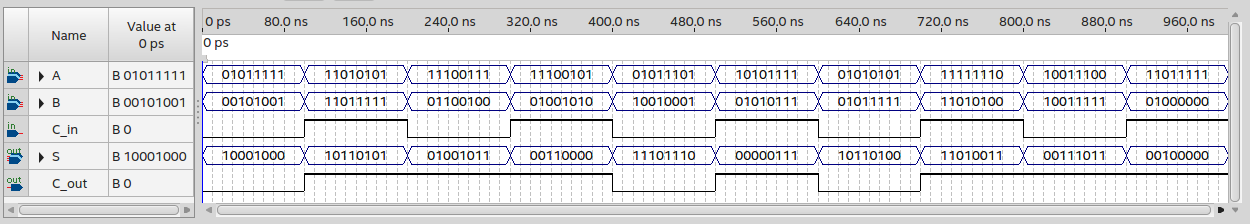
\includegraphics[width=\linewidth]{images/lab5-3-8bit-1-bin.png}
        \caption{Values represented in binary.}\label{fig:lab5-3-8bit-1-bin}
    \end{subfigure}
    \\[1cm]
    \begin{subfigure}{\linewidth}
       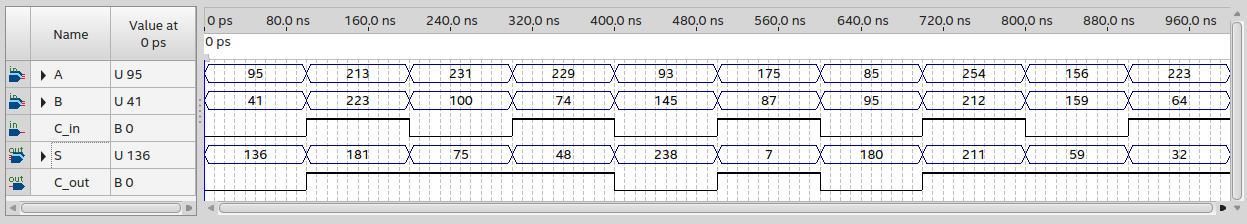
\includegraphics[width=\linewidth]{images/lab5-3-8bit-1-dec.png}
       \caption{Values represented in decimal.}\label{fig:lab5-3-8bit-1-dec}
    \end{subfigure}
    \caption{Test signal results for the 8-bit adder circuit.}\label{fig:lab5-3-8bit-1}
\end{figure}
\end{landscape}

\section*{Conclusion}

This lab illustrated the process of designing large combinational circuits by combining smaller logical units. Basic half-adder and full-adder circuits were implemented using Quartus and were tested by mapping them onto a FPGA board. These circuits were then used to develop an 8-bit adder circuit, which was verified using simulation software. Common issues when designing combinational circuits such as carry propagation and delay were considered and addressed during lab assignments. 

A possible extension for this lab would be using the implemented 8-bit adder circuit to design a higher-precision adder, such as a 32-bit or 64-bit adder. Additionally, during this lab, no requirements were imposed on the design of the adder circuits other that their terminal behavior. Therefore this lab might be further extended by introducing constraints to the circuit design process such as minimizing time complexity or power consumption.

\FloatBarrier

\bibliography{../ecee-2160-common.bib,./ecee-2160-lab-5.bib}

\bibliographystyle{unsrt}


\end{document}